% Copyright 2020-2023 Robert Bosch GmbH

% Licensed under the Apache License, Version 2.0 (the "License");
% you may not use this file except in compliance with the License.
% You may obtain a copy of the License at

% http://www.apache.org/licenses/LICENSE-2.0

% Unless required by applicable law or agreed to in writing, software
% distributed under the License is distributed on an "AS IS" BASIS,
% WITHOUT WARRANTIES OR CONDITIONS OF ANY KIND, either express or implied.
% See the License for the specific language governing permissions and
% limitations under the License.

This chapter explains the features of the \pkg\ in detail.

\section{How to execute}

The \pkg\ is implemented in Python3 and therefore requires a Python3 installation.

A basic Python script to use the \pkg\ can look like this:

\begin{pythoncode}
from JsonPreprocessor.CJsonPreprocessor import CJsonPreprocessor
import pprint

json_preprocessor = CJsonPreprocessor()
try:
   values = json_preprocessor.jsonLoad("./file.jsonp")
   pprint.pprint(values)
except Exception as reason:
   print(f"'{reason}'")
\end{pythoncode}

\textbf{!!! Caution:} relative path bug:
\href{https://github.com/test-fullautomation/python-jsonpreprocessor/issues/83}{issues/83} \textbf{!!!}

The main method of the \pkg\ is: \pcode{jsonLoad}. Input is the path and the name of a JSON file.
Output is a dictionary containing all values parsed from this JSON file.

In case of any errors while computing the JSON file, the \pkg\ throws an exception. Therefore it is required
to call the method \pcode{jsonLoad} inside a \pcode{try/except} block.

\pcode{pprint} is used in this example to give the output a better readibility in console.

In the following sections we concentrate on the content of the JSON files and the corresponding results.

The way to get these results is in every case the same: the example script listed above.


% --------------------------------------------------------------------------------------------------------------

\section{Standard JSON format}

The \pkg\ supports JSON files with standard extension \plog{.json} and standard content.

\textbullet\ JSON file:

\begin{pythoncode}
{
   "param1" : "value1",
   "param2" : "value2"
}
\end{pythoncode}

\textbf{Outcome:}

\begin{pythonlog}
{'param1': 'value1', 'param2': 'value2'}
\end{pythonlog}

A JSON file with extension \plog{.jsonp} and same content will produce the same output.

We recommend to give every JSON file the extension \plog{.jsonp} to have a strict separation between the standard and the extended JSON format.

The following example still contains standard JSON content, but with parameters of several different data types (simple and composite).

\begin{pythoncode}
{
   "param_01" : "string",
   "param_02" : 123,
   "param_03" : 4.56,
   "param_04" : ["A", "B", "C"],
   "param_05" : {"A" : 1, "B" : 2, "C" : 3}
}
\end{pythoncode}

This content produces the following output:

\begin{pythonlog}
{'param_01': 'string',
 'param_02': 123,
 'param_03': 4.56,
 'param_04': ['A', 'B', 'C'],
 'param_05': {'A': 1, 'B': 2, 'C': 3}}
\end{pythonlog}


% --------------------------------------------------------------------------------------------------------------

\section{Boolean and null values}

JSON supports the boolean values \pcode{true} and \pcode{false}, and also the null value \pcode{null}.

In Python the corresponding values are different: \pcode{True}, \pcode{False} and \pcode{None}.

Because the \pkg\ is a Python application and therefore the returned content is required to be formatted Python compatible,
the \pkg\ does a conversion automatically.

Accepted in JSON files are both styles:

\begin{pythoncode}
{
   "param_06" : true,
   "param_07" : false,
   "param_08" : null,
   "param_09" : True,
   "param_10" : False,
   "param_11" : None
}
\end{pythoncode}

But the usage of Python keywords (\pcode{param_09} - \pcode{param_11}) requires a small extension of the example above.
The initialization of the \pkg\ needs to set the syntax to Python (\pcode{syntax="python"}):

\begin{pythoncode}
json_preprocessor = CJsonPreprocessor(syntax="python")
\end{pythoncode}

Without setting the syntax to Python, the usage of Python keywords within JSON files causes an exception.

\textbf{!!! Caution}: This will be changed:
\href{https://github.com/test-fullautomation/python-jsonpreprocessor/issues/84}{issues/84} \textbf{!!!}

The output contains all keywords in Python style only:

\begin{pythonlog}
{'param_06': True,
 'param_07': False,
 'param_08': None,
 'param_09': True,
 'param_10': False,
 'param_11': None}
\end{pythonlog}


% --------------------------------------------------------------------------------------------------------------

\newpage

\section{Comments}

Comments can be added to JSON files with \pcode{//}:

\begin{pythoncode}
{
   // JSON keywords
   "param_06" : true,
   "param_07" : false,
   "param_08" : null,
   // Python keywords
   "param_09" : True,
   "param_10" : False,
   "param_11" : None
}
\end{pythoncode}

All lines starting with \pcode{//}, are ignored by the \pkg. The output of this example is the same than in the previous example.


% --------------------------------------------------------------------------------------------------------------

\newpage

\section{Import of JSON files}

We assume the following scenario:

A software component \textit{A} requires a set of configuration parameters. A software component \textit{B} that belongs to the same
main software or to the same project, requires another set of configuration parameters. Additionally both components
require a common set of parameters (with the same values).

The outcome is that at least we need two JSON configuration files:

\begin{enumerate}
   \item A file \plog{componentA.jsonp} containing all parameters required for component \textit{A}
   \item A file \plog{componentB.jsonp} containing all parameters required for component \textit{B}
\end{enumerate}

But with this solution both JSON files would contain also the common set of parameters. This is unfavorable, because
the corresponding values need to be maintained at two different positions.

Therefore we extend the list of JSON files by a file containing the common part only:

\begin{enumerate}
   \item A file \plog{common.jsonp} containing all parameters that are the same for component \textit{A} and component \textit{B}
   \item A file \plog{componentA.jsonp} containing all parameters required for component \textit{A}
   \item A file \plog{componentB.jsonp} containing all parameters required for component \textit{B}
\end{enumerate}

Finally we use the import mechanism of the \pkg\ to import the file \plog{common.jsonp} in file \plog{componentA.jsonp} and also in
file \plog{componentB.jsonp}.

\vspace{2ex}

This can be the content of the JSON files:

\vspace{2ex}

\textbullet \plog{common.jsonp}

\begin{pythoncode}
{
   // common parameters
   "common_param_1" : "common value 1",
   "common_param_2" : "common value 2"
}
\end{pythoncode}

\textbullet \plog{componentA.jsonp}

\begin{pythoncode}[linebackgroundcolor=\hlcode{3}]
{
   // common parameters
   "[import]" : "./common.jsonp",
   //
   // component A parameters
   "componentA_param_1" : "componentA value 1",
   "componentA_param_2" : "componentA value 2"
}
\end{pythoncode}

\textbullet \plog{componentB.jsonp}

\begin{pythoncode}[linebackgroundcolor=\hlcode{3}]
{
   // common parameters
   "[import]" : "./common.jsonp",
   //
   // component B parameters
   "componentB_param_1" : "componentB value 1",
   "componentB_param_2" : "componentB value 2"
}
\end{pythoncode}

\textbf{Explanation:}

\vspace{2ex}

JSON files are imported with the key \pcode{"[import]"}. The value of this key is the path and name of the JSON file to be imported.

A JSON file can contain more than one import. Imports can be nested: An imported JSON file can import further JSON files also.

\newpage

\textbf{Outcome:}

The file \plog{componentA.jsonp} produces the following output:

\begin{pythonlog}
{'common_param_1': 'common value 1',
 'common_param_2': 'common value 2',
 'componentA_param_1': 'componentA value 1',
 'componentA_param_2': 'componentA value 2'}
\end{pythonlog}

The file \plog{componentB.jsonp} produces the following output:

\begin{pythonlog}
{'common_param_1': 'common value 1',
 'common_param_2': 'common value 2',
 'componentB_param_1': 'componentB value 1',
 'componentB_param_2': 'componentB value 2'}
\end{pythonlog}

It can be seen that the returned dictionary contains both the parameters from the loaded JSON file and the parameters imported by the loaded JSON file.


% --------------------------------------------------------------------------------------------------------------

\section{Overwrite parameters}

We take over the scenario from the previous section: We still have a JSON file \plog{componentA.jsonp} containig the parameters for
component \textit{A}, a JSON file \plog{componentB.jsonp} for component \textit{B} and a JSON file \plog{common.jsonp} for both components.

But now component \textit{B} requires a different value of a common parameter: Within a JSON file we need to change the value of a parameter
that is initialized within an imported file. That is possible.

\vspace{2ex}

This is now the content of the JSON files:

\vspace{2ex}

\textbullet \plog{common.jsonp}

\begin{pythoncode}
{
   // common parameters
   "common_param_1" : "common value 1",
   "common_param_2" : "common value 2"
}
\end{pythoncode}

\textbullet \plog{componentA.jsonp}

\begin{pythoncode}
{
   // common parameters
   "[import]" : "./common.jsonp",
   //
   // component A parameters
   "componentA_param_1" : "componentA value 1",
   "componentA_param_2" : "componentA value 2"
}
\end{pythoncode}

\textbullet \plog{componentB.jsonp}

\begin{pythoncode}[linebackgroundcolor=\hlcode{8,9}]
{
   // common parameters
   "[import]" : "./common.jsonp",
   //
   // component B parameters
   "componentB_param_1" : "componentB value 1",
   "componentB_param_2" : "componentB value 2",
   // overwrite parameter initialized by imported file
   "common_param_2" : "common componentB value 2"
}
\end{pythoncode}

\newpage

\textbf{Explanation:}

\vspace{2ex}

With

\begin{pythoncode}
   "common_param_2" : "common componentB value 2"
\end{pythoncode}

in \plog{componentB.jsonp} the initial definition

\begin{pythoncode}
   "common_param_2" : "common value 2"
\end{pythoncode}

in \plog{common.jsonp} is overwritten.

\vspace{2ex}

\textbf{Outcome:}

\vspace{2ex}

The file \plog{componentB.jsonp} produces the following output:

\begin{pythonlog}
{'common_param_1': 'common value 1',
 'common_param_2': 'common componentB value 2',
 'componentB_param_1': 'componentB value 1',
 'componentB_param_2': 'componentB value 2'}
\end{pythonlog}

\vspace{2ex}

Important: \textit{The value a parameter has finally, depends on the order of definitions, redefinitions and imports!}

\vspace{2ex}

In file \plog{componentB.jsonp} we move the import of \plog{common.jsonp} to the bottom:

\begin{pythoncode}[linebackgroundcolor=\hlcode{8}]
{
   // component B parameters
   "componentB_param_1" : "componentB value 1",
   "componentB_param_2" : "componentB value 2",
   "common_param_2" : "common componentB value 2"
   //
   // common parameters
   "[import]" : "./common.jsonp",
}
\end{pythoncode}

Now the imported file overwrites the value initialized in the importing file.

\vspace{2ex}

\textbf{Outcome:}

\vspace{2ex}

\begin{pythonlog}
{'common_param_1': 'common value 1',
 'common_param_2': 'common value 2',
 'componentB_param_1': 'componentB value 1',
 'componentB_param_2': 'componentB value 2'}
\end{pythonlog}

\vspace{2ex}

Up to now we considered simple data types only. In case we want to overwrite a parameter that is part of a composite data type, we need to extend the syntax.
This is explained in the next examples.

\vspace{2ex}

Again we take over the scenario from the previous section: We still have a JSON file \plog{componentA.jsonp} containig the parameters for
component \textit{A}, a JSON file \plog{componentB.jsonp} for component \textit{B} and a JSON file \plog{common.jsonp} for both components.

But now all values are part of composite data types like lists and dictionaries.

This is the content of the JSON files:

\vspace{2ex}

\textbullet \plog{common.jsonp}

\begin{pythoncode}
{
   // common parameters
   "common_param_1" : ["common value 1.1", "common value 1.2"],
   "common_param_2" : {"common_key_2_1" : "common value 2.1" ,
                       "common_key_2_2" : "common value 2.2"}
}
\end{pythoncode}

\textbullet \plog{componentA.jsonp}

\begin{pythoncode}
{
   // common parameters
   "[import]" : "./common.jsonp",
   //
   // component A parameters
   "componentA_param_1" : ["componentA value 1.1", "componentA value 1.2"],
   "componentA_param_2" : {"componentA_key_2_1" : "componentA value 2.1" ,
                           "componentA_key_2_2" : "componentA value 2.2"}
}
\end{pythoncode}

\textbullet \plog{componentB.jsonp}

\begin{pythoncode}
{
   // common parameters
   "[import]" : "./common.jsonp",
   //
   // component B parameters
   "componentB_param_1" : ["componentB value 1.1", "componentB value 1.2"],
   "componentB_param_2" : {"componentB_key_2_1" : "componentB value 2.1" ,
                           "componentB_key_2_2" : "componentB value 2.2"}
}
\end{pythoncode}

Like in previous examples, the outcome is a merge of the imported JSON file and the importing JSON file, e.g. for \plog{componentA.jsonp}:

\begin{pythonlog}
{'common_param_1': ['common value 1.1', 'common value 1.2'],
 'common_param_2': {'common_key_2_1': 'common value 2.1',
                    'common_key_2_2': 'common value 2.2'},
 'componentA_param_1': ['componentA value 1.1', 'componentA value 1.2'],
 'componentA_param_2': {'componentA_key_2_1': 'componentA value 2.1',
                        'componentA_key_2_2': 'componentA value 2.2'}}
\end{pythonlog}

\vspace{2ex}

Now the following questions need to be answered:

\begin{enumerate}
   \item How to get the value of an already existing parameter?
   \item How to get the value of a single element of a parameter of nested data type (list, dictionary)?
   \item How to overwrite the value of a single element of a parameter of nested data type?
   \item How to add an element to a parameter of nested data type?
\end{enumerate}

We introduce another JSON file \plog{componentB.2.jsonp} in which we import the JSON file \plog{componentB.jsonp}.
In this file we also add content to work with simple and composite data types to answer the questions above.

\newpage

This is the initial content of \plog{componentB.2.jsonp}:

\begin{pythoncode}
{
   // import of componentB parameters
   "[import]" : "./componentB.jsonp",
   //
   // some additional parameters of simple data type
   "string_val" : "ABC",
   "int_val"    : 123,
   "float_val"  : 4.56,
   "bool_val"   : true,
   "null_val"   : null,

   // access to existing parameters
   "string_val_b"         : ${string_val},
   "int_val_b"            : ${int_val},
   "float_val_b"          : ${float_val},
   "bool_val_b"           : ${bool_val},
   "null_val_b"           : ${null_val},
   "common_param_1_b"     : ${common_param_1},
   "componentB_param_2_b" : ${componentB_param_2}
}
\end{pythoncode}

\vspace{2ex}

\textbf{The rules for accessing parameters are:}

\begin{itemize}
   \item Existing parameters are accessed by a dollar operator and a pair of curly brackets (\pcode{$\{...\}}) with the parameter name inside.
   \item If the entire expression of the right hand side of the colon is such a dollar operator expression, the entire expression must \textit{not}
         be encapsulated in quotes. 
   \item The dollar operator keeps the data type of the referenced parameter.
\end{itemize}

\textbf{Outcome:}

\vspace{2ex}

\begin{pythonlog}
{'bool_val': True,
 'bool_val_b': True,
 'common_param_1': ['common value 1.1', 'common value 1.2'],
 'common_param_1_b': ['common value 1.1', 'common value 1.2'],
 'common_param_2': {'common_key_2_1': 'common value 2.1',
                    'common_key_2_2': 'common value 2.2'},
 'componentB_param_1': ['componentB value 1.1', 'componentB value 1.2'],
 'componentB_param_2': {'componentB_key_2_1': 'componentB value 2.1',
                        'componentB_key_2_2': 'componentB value 2.2'},
 'componentB_param_2_b': {'componentB_key_2_1': 'componentB value 2.1',
                          'componentB_key_2_2': 'componentB value 2.2'},
 'float_val': 4.56,
 'float_val_b': 4.56,
 'int_val': 123,
 'int_val_b': 123,
 'null_val': None,
 'null_val_b': None,
 'string_val': 'ABC',
 'string_val_b': 'ABC'}
\end{pythonlog}

Let's take a deeper look at the following line:

\begin{pythoncode}
"int_val_b"            : ${int_val},
\end{pythoncode}

Like mentioned in the rules above, the dollar operator keeps the data type of the referenced parameter:
In case of \pcode{int_val} is of type \pcode{int}, also \pcode{int_val_b} will be of type \pcode{int}.

\newpage

Like mentioned in the rules above, dollar operator expressions must \textit{not} be encapsulated in quotes.
But nevertheless it is possible to use quotes. In case of:

\begin{pythoncode}
"int_val_b"            : "${int_val}",
\end{pythoncode}

the parameter \pcode{int_val_b} would be of type \pcode{string}.

\vspace{2ex}

\textbf{Value of a single element of a parameter of nested data type}

To access an element of a list and a key of a dictionary, we change the content of file \plog{componentB.2.jsonp} to:

\begin{pythoncode}
{
   // import of componentB parameters
   "[import]" : "./componentB.jsonp",
   //
   "list_element_0" : "${componentB_param_1}[0]",
   "dict_key_2_2"   : ${common_param_2}['common_key_2_2']
}
\end{pythoncode}

\textbf{!!! CAUTION}: Code neeeds to be adapted (remove quotes) after
\href{https://github.com/test-fullautomation/python-jsonpreprocessor/issues/85}{issues/85}
is resolved \textbf{!!!}

\textbf{Outcome:}

\vspace{2ex}

\begin{pythonlog}
{'common_param_1': ['common value 1.1', 'common value 1.2'],
 'common_param_2': {'common_key_2_1': 'common value 2.1',
                    'common_key_2_2': 'common value 2.2'},
 'componentB_param_1': ['componentB value 1.1', 'componentB value 1.2'],
 'componentB_param_2': {'componentB_key_2_1': 'componentB value 2.1',
                        'componentB_key_2_2': 'componentB value 2.2'},
 'dict_key_2_2': 'common value 2.2',
 'list_element_0': 'componentB value 1.1'}
\end{pythonlog}

\vspace{2ex}

\textbf{Overwrite the value of a single element of a parameter of nested data type}

In the next example we overwrite the value of a list element and the value of a dictionary key.

Again we change the content of file \plog{componentB.2.jsonp}:

\begin{pythoncode}
{
   // import of componentB parameters
   "[import]" : "./componentB.jsonp",
   //
   ${componentB_param_1}[0]            : "componentB value 1.1 (new)",
   ${common_param_2}['common_key_2_1'] : "common value 2.1 (new)"
}
\end{pythoncode}

The dollar operator syntax at the left hand side of the colon is the same than previously used on the right hand side.
The entire expression must \textit{not} be encapsulated in quotes.

\textbf{Outcome:}

The single elements of the list and the dictionary are updated, all other elements are unchanged.

\vspace{2ex}

\begin{pythonlog}
{'common_param_1': ['common value 1.1', 'common value 1.2'],
 'common_param_2': {'common_key_2_1': 'common value 2.1 (new)',
                    'common_key_2_2': 'common value 2.2'},
 'componentB_param_1': ['componentB value 1.1 (new)', 'componentB value 1.2'],
 'componentB_param_2': {'componentB_key_2_1': 'componentB value 2.1',
                        'componentB_key_2_2': 'componentB value 2.2'}}
\end{pythonlog}

\newpage

\textbf{Add an element to a parameter of nested data type}

Adding further elements to an already existing list is not possible in JSON! But it is possible to add keys to
an already existing dictionary.

The following example extends the dictionary \pcode{common_param_2} by an additional key \pcode{common_key_2_3}:

\begin{pythoncode}
{
   // import of componentB parameters
   "[import]" : "./componentB.jsonp",
   //
   ${common_param_2}['common_key_2_3'] : "common value 2.3"
}
\end{pythoncode}

\textbf{Outcome:}

\vspace{2ex}

\begin{pythonlog}
{'common_param_1': ['common value 1.1', 'common value 1.2'],
 'common_param_2': {'common_key_2_1': 'common value 2.1',
                    'common_key_2_2': 'common value 2.2',
                    'common_key_2_3': 'common value 2.3'},
 'componentB_param_1': ['componentB value 1.1', 'componentB value 1.2'],
 'componentB_param_2': {'componentB_key_2_1': 'componentB value 2.1',
                        'componentB_key_2_2': 'componentB value 2.2'}}
\end{pythonlog}

\vspace{2ex}

\textbf{Use of a common dictionary}

\vspace{2ex}

The last example in this section covers the following use case:

\begin{itemize}
   \item We have several JSON files, each for a certain purpose within a project (e.g. for every feature of this project a separate JSON file).
   \item They belong together and therefore they are all imported into a main JSON file that is the file that is handed over to the \pkg.
   \item Every imported JSON file introduces a certain bunch of parameters. All parameters need to be a part of a common dictionary.
   \item Outcome is that finally only one single dictionary is used to access the parameters from all JSON files imported in the main JSON file.
\end{itemize}

To realize this, it is necessary to separate the initialization of the dictionary from all positions where keys are added to this dictionary.

These are the JSON files:

\vspace{2ex}

\textbullet \plog{project.jsonp}

\begin{pythoncode}
{
   // initialization
   "project_values" : {},
   //
   // add some common values
   ${project_values}['common_project_param_1'] : "common project value 1",
   ${project_values}['common_project_param_2'] : "common project value 2",
   //
   // import feature parameters
   "[import]" : "./featureA.jsonp",
   "[import]" : "./featureB.jsonp",
   "[import]" : "./featureC.jsonp"
}
\end{pythoncode}

\newpage

\textbullet \plog{featureA.jsonp}

\begin{pythoncode}
{
   // parameters required for feature A
   ${project_values}['featureA_params'] : {},
   ${project_values}['featureA_params']['featureA_param_1'] : "featureA param 1 value",
   ${project_values}['featureA_params']['featureA_param_2'] : "featureA param 2 value"
}
\end{pythoncode}

\vspace{2ex}

\textbullet \plog{featureB.jsonp}

\begin{pythoncode}
{
   // parameters required for feature B
   ${project_values}['featureB_params'] : {},
   ${project_values}['featureB_params']['featureB_param_1'] : "featureB param 1 value",
   ${project_values}['featureB_params']['featureB_param_2'] : "featureB param 2 value"
}
\end{pythoncode}

\vspace{2ex}

\textbullet \plog{featureC.jsonp}

\begin{pythoncode}
{
   // parameters required for feature C
   ${project_values}['featureC_params'] : {},
   ${project_values}['featureC_params']['featureC_param_1'] : "featureC param 1 value",
   ${project_values}['featureC_params']['featureC_param_2'] : "featureC param 2 value"
}
\end{pythoncode}

\vspace{2ex}

\textbf{Explanation:}

\vspace{2ex}

Every \plog{feature*.jsonp} file refer to the dictionary inizialized within \plog{project.jsonp}.

Important is that the initialization \pcode{"project_values" : \{\},} happens at top level (\plog{project.jsonp}),
and not within the imported files (\plog{feature*.jsonp}), otherwise follow up initializations would delete
previously added keys of this dictionary!

\vspace{2ex}

\textbf{Outcome:}

\vspace{2ex}

\begin{pythonlog}
{'project_values': {'common_project_param_1': 'common project value 1',
                    'common_project_param_2': 'common project value 2',
                    'featureA_params': {'featureA_param_1': 'featureA param 1 value',
                                        'featureA_param_2': 'featureA param 2 value'},
                    'featureB_params': {'featureB_param_1': 'featureB param 1 value',
                                        'featureB_param_2': 'featureB param 2 value'},
                    'featureC_params': {'featureC_param_1': 'featureC param 1 value',
                                        'featureC_param_2': 'featureC param 2 value'}}}
\end{pythonlog}


% --------------------------------------------------------------------------------------------------------------

\newpage

\section{\texttt{dotdict} notation}

Up to now we have accessed dictionary keys in this way (standard notation):

\begin{pythoncode}
${dictionary}['key']['sub_key']
\end{pythoncode}

Additionally to this standard notation, the \pkg\ supports the so called \textit{dotdict} notation where keys
are handled as attributes:

\begin{pythoncode}
${dictionary.key.sub_key}
\end{pythoncode}

In standard notation keys are encapsulated in square brackets and all together is placed \textit{outside} the curly brackets.
In dotdict notation the dictionary name and the keys are separated by dots from each other. All together is placed \textit{inside}
the curly brackets.

In standard notation key names are allowed to contain dots:

\begin{pythoncode}
${dictionary}['key']['sub.key']
\end{pythoncode}

In dotdict notation this would cause ambiguities:

\begin{pythoncode}
${dictionary.key.sub.key}
\end{pythoncode}

Therefore it is not possible to implement in this way! In case you need to have dots inside key names, you must use the standard notation.
We recommend to prefer underlines as separator - like done in the examples in this document.

\textit{Do you really need dots inside key names?}

Please keep in mind: The dotdict notation is a reduced one. Because of parts are missing (e.g. the single quotes around key names),
the outcome can be code that is really hard to capture.

In the following example we create a composite data structure and demonstate how to access single elements in both notations.

\vspace{2ex}

\textbullet\ JSON file:

\begin{pythoncode}
{
   // composite data structure
   "params" : [{"dict_1_key_1" : "dict_1_key_1 value",
                "dict_1_key_2" : ["dict_1_key_2 value 1", "dict_1_key_2 value 2"]},
               //
               {"dict_2_key_1" : "dict_2_key_1 value",
                "dict_2_key_2" : {"dict_2_A_key_1" : "dict_2_A_key_1 value",
                                  "dict_2_A_key_2" : ["dict_2_A_key_2 value 1", "dict_2_A_key_2 value 2"]}}],
   //
   // access to single elements of composite data structure
   //
   // a) standard notation
   "dict_1_key_2_value_2_standard" : ${params}[0]['dict_1_key_2'][1],
   // b) dotdict notation
   // "dict_1_key_2_value_2_dotdict" : ${params.0.dict_1_key_2.1},
   // -> 'The variable '${params}['0']['dict_1_key_2']['1']' is not available!'
   //
   // c) standard notation
   "dict_2_A_key_2_value_2_standard" : ${params}[1]['dict_2_key_2']['dict_2_A_key_2'][1]
   // d) dotdict notation
   // "dict_2_A_key_2_value_2_dotdict" : ${params.1.dict_2_key_2.dict_2_A_key_2.1}
   // -> 'The variable '${params}['1']['dict_2_key_2']['dict_2_A_key_2']['1']' is not available!'
}
\end{pythoncode}

\textbf{!!! Caution:} dotdict bug:
\href{https://github.com/test-fullautomation/python-jsonpreprocessor/issues/89}{issues/89} \textbf{!!!}

\newpage

\textbf{Outcome:}

In case of the composite data structure becomes more and more nested (and if also the key names contain numbers), understanding
the expressions (like \pcode{$\{params.1.dict_2_key_2.dict_2_A_key_2.1\}}) becomes more and more challenging!

\vspace{2ex}

\begin{pythonlog}
{'dict_1_key_2_value_2_standard': 'dict_1_key_2 value 2',
 'dict_2_A_key_2_value_2_standard': 'dict_2_A_key_2 value 2',
 'params': [{'dict_1_key_1': 'dict_1_key_1 value',
             'dict_1_key_2': ['dict_1_key_2 value 1', 'dict_1_key_2 value 2']},
            {'dict_2_key_1': 'dict_2_key_1 value',
             'dict_2_key_2': {'dict_2_A_key_1': 'dict_2_A_key_1 value',
                              'dict_2_A_key_2': ['dict_2_A_key_2 value 1',
                                                 'dict_2_A_key_2 value 2']}}]}
\end{pythonlog}

% --------------------------------------------------------------------------------------------------------------
% === to be reworked and extended after issued are solved
% --------------------------------------------------------------------------------------------------------------


% --------------------------------------------------------------------------------------------------------------

\newpage

\section{Substitution of dollar operator expressions}

Like shown in previous examples, existing parameters are accessed by a dollar operator and a pair of curly brackets (\pcode{$\{...\}}) with the parameter name inside.

We discussed use cases, where the entire expression of the left hand side of the colon and also the entire expression of the right hand side of the colon
have been either hard coded strings, encapsulated in quotes, or dollar operator expressions, not encapsulated in quotes.

Also a mix of both is possible!

Outcome is a hard coded string, encapsulated in quotes, with parts represented by one or more than one dollar operator expression. This can be used to create
new content very dynamically: On the right hand side of the colon new string values can be created; on the left hand side of the colon this mechanism
generates dynamic parameter names.

\vspace{2ex}

\textbullet\ JSON file:

\begin{pythoncode}
{
   "project"     : "Test",
   "version"     : 1.23,
   "item_number" : 1,
   "component"   : "componentA",
   //
   "${project}_message_${item_number}" : "Component '${component}' has version ${version}"
}
\end{pythoncode}

\vspace{2ex}

\textbf{Outcome:}

\begin{pythonlog}
{'component': 'componentA',
 'item_number': 1,
 'project': 'Test',
 'project)_message_str(1': "Component 'componentA' has version 1.23",
 'version': 1.23}
\end{pythonlog}

\textbf{!!! Caution:} substitution bug:
\href{https://github.com/test-fullautomation/python-jsonpreprocessor/issues/91}{issues/91} \textbf{!!!}

\textit{We recommend to use simple data types for this kind of substitution only!}

But nevertheless, on the right hand side of the colon also composite data types are possible. Here it might makes sense to use them.
But on the left hand side of the colon only simple data types are allowed. Because it makes no sense to create
parameter names based on composite data types. Most probably this would cause invalid key names.

To demonstrate this, we change the JSON file to:

\begin{pythoncode}
{
   "component"      : "componentA",
   "composite_data" : ["AB", 12, True, null, {"kA" : "kAval", "kB" : "kBval"}],
   //
   "test_parameter" : "Key values of component '${component}' are ${composite_data}"
}
\end{pythoncode}

\textbf{!!! Caution:} substitution bug:
\href{https://github.com/test-fullautomation/python-jsonpreprocessor/issues/92}{issues/92} \textbf{!!!}

Not working currently:
\begin{pythoncode}
   "test_parameter" : "Key values of component '${component}' are: ${composite_data}"
\end{pythoncode}

\vspace{2ex}

\textbf{Outcome:}

\begin{pythonlog}
{'component': 'componentA',
 'composite_data': ['AB', 12, True, None, {'kA': 'kAval', 'kB': 'kBval'}],
 'test_parameter': "Key values of component 'componentA' are ['AB', 12, True, "
                   "None, {'kA': 'kAval', 'kB': 'kBval'}]"}
\end{pythonlog}

\newpage

Now we try to do the same on the left hand side of the colon:

\begin{pythoncode}
{
   "value"          : "string value",
   "composite_data" : ["AB", 12, True, null, {"kA" : "kAval", "kB" : "kBval"}],
   //
   "test_parameter_${composite_data}" : ${value}
}
\end{pythoncode}

\vspace{2ex}

\textbf{Outcome:}

\begin{pythonlog}
!!! Error message expected; still under development !!!
\end{pythonlog}

\textbf{!!! Caution:}
\href{https://github.com/test-fullautomation/python-jsonpreprocessor/issues/69#issuecomment-1589581903}{issues/69 issuecomment-1589581903} \textbf{!!!}


% --------------------------------------------------------------------------------------------------------------

\newpage

\section{Implicite creation of dictionaries}

Up to now we have discussed two different ways of creating nested dictionaries.

The first one is \q{on the fly}, like:

\begin{pythoncode}
{
   "project_values" : {"keyA" : "keyA value",
                       "keyB" : {"keyB1" : "keyB1 value",
                                 "keyB2" : {"keyB21" : "keyB21 value",
                                            "keyB22" : "keyB22 value"}}}
}
\end{pythoncode}

In case of it is required to split the definition into several files, we have to add keys (and also the initialization) line by line:

\begin{pythoncode}
{
   "project_values" : {},
   ${project_values}['keyA'] : "keyA value",
   ${project_values}['keyB'] : {},
   ${project_values}['keyB']['keyB1'] : "keyB1 value",
   ${project_values}['keyB']['keyB2'] : {},
   ${project_values}['keyB']['keyB2']['keyB21'] : "keyB21 value",
   ${project_values}['keyB']['keyB2']['keyB22'] : "keyB22 value"
}
\end{pythoncode}

The result will be the same as in the previous example.

It can be seen now that this way of creating nested dictionaries is rather long winded, because every inititialization of a dictionary
requires a separate line of code (at every level).

To shorten the code, the \pkg\ supports an implicite creation of dictionaries.

This is the resulting code in standard notation:

\begin{pythoncode}
{
   ${project_values}['keyA'] : "keyA value",
   ${project_values}['keyB']['keyB1'] : "keyB1 value",
   ${project_values}['keyB']['keyB2']['keyB21'] : "keyB21 value",
   ${project_values}['keyB']['keyB2']['keyB22'] : "keyB22 value"
}
\end{pythoncode}

\vspace{2ex}

And the same in dotdict notation (with precondition, that no key name contains a dot):

\begin{pythoncode}
{
   ${project_values.keyA} : "keyA value",
   ${project_values.keyB.keyB1} : "keyB1 value",
   ${project_values.keyB.keyB2.keyB21} : "keyB21 value",
   ${project_values.keyB.keyB2.keyB22} : "keyB22 value"
}
\end{pythoncode}

\vspace{2ex}

\textbf{Caution:}

We urgently recommend \textit{not} to mixup both styles in one line of code. In case of keys contain a list and also numerical indices are involved,
we recommend to prefer the standard notation. 

Please be aware of: In case of a missing level in between an expression like 

\begin{pythoncode}
{
   ${project_values.keyB.keyB2.keyB22} : "keyB22 value"
}
\end{pythoncode}

you will \textit{not} get an error message! The entire data structure will be created implicitely. The impact is that this method
is very susceptible to typing mistakes.

The implicite creation of data structures does not work with lists! In case you use a list index out of range, you will get
a corresponding error message.


% --------------------------------------------------------------------------------------------------------------

\newpage

\section{VSCodium support}

Above we mentioned that the JSON syntax extensions introduced by the \pkg, harm the syntax highlighting of editors.

Either we give the JSON files the extension \pcode{.json}, then an editor expects a JSON file in standard syntax,
or we change the extension to \pcode{.jsonp}, but in this case an editor usually does not know how to display a file of such type.

In case you use \href{https://vscodium.com/}{VSCodium}, you can install a
\href{https://github.com/test-fullautomation/vscode-jsonp}{jsonp extension}. 

With this extension the VSCodium editor will be able to display \pcode{.jsonp} files properly.

\vspace{2ex}

\textbf{Some Impressions:}

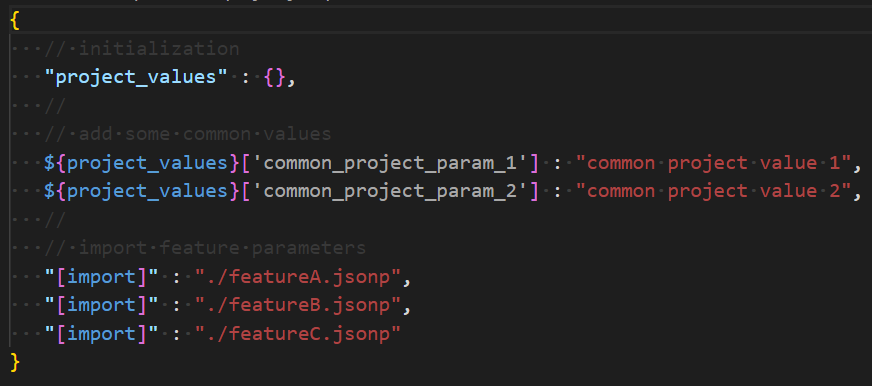
\includegraphics{./pictures/screenshot1.png}

\vspace{2ex}

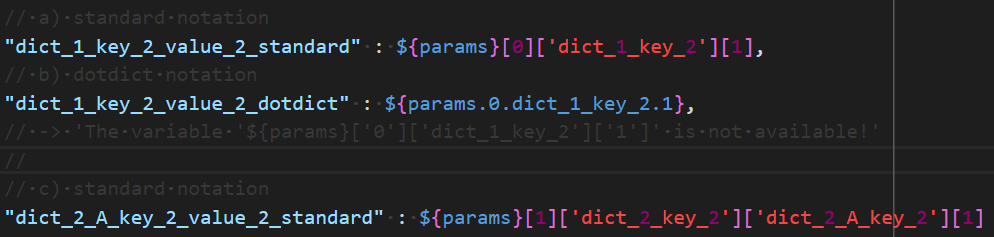
\includegraphics{./pictures/screenshot2.png}



% --------------------------------------------------------------------------------------------------------------
% TODO:
% - extended use of nested parameters
% --------------------------------------------------------------------------------------------------------------




